%% Font size %%
\documentclass[11pt]{article}

%% Load the custom package
\usepackage{Mathdoc}

%% Numéro de séquence %% Titre de la séquence %%
\renewcommand{\centerhead}{DS1 - Pythagore : Calcul d’Hypoténuse}

%% Spacing commands %%
\renewcommand{\baselinestretch}{1} \setlength{\parindent}{0pt}

\begin{document}

\entetedevoirs{10}

\begin{center}
%\duree{30 minutes} 
\coefficient{0,5}
\calculatrice{1}
%\copieseparee{0}
\end{center}


\begin{exercicedevoir}[5]
\begin{center}
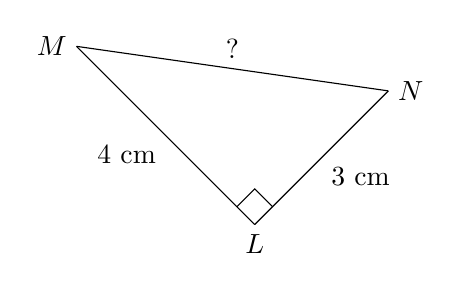
\begin{tikzpicture}[scale=0.4,rotate=45]
\coordinate (A) at (0,0); \coordinate (B) at (6,0); \coordinate (C) at
(0,8);

\draw (A) -- (B) node[midway,below right] {3 cm}; \draw (A) -- (C)
node[midway,below left] {4 cm}; \draw (B) -- (C) node[midway,above]
{$?$};

\node[below] at (A) {$L$}; \node[right] at (B) {$N$};
\node[left] at (C) {$M$};

% Angle droit en A
\draw (0.8,0) -- (0.8,0.8) -- (0,0.8);
\end{tikzpicture}
\end{center}

\begin{enumerate}
\item \textbf{Égalité de Pythagore :} \\
\item \textbf{Remplacement :} \\
\item \textbf{Calcul de la racine :} \\
\item \textbf{Phrase réponse :} \\
\end{enumerate}
\end{exercicedevoir}

\vfill

\begin{exercicedevoir}[5]
\begin{center}
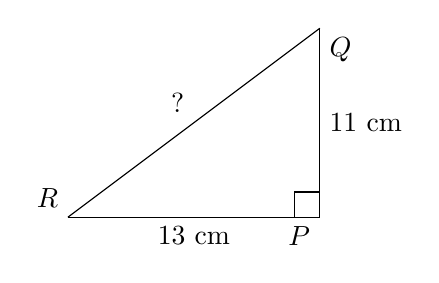
\begin{tikzpicture}[scale=0.4,rotate=90]
\coordinate (A) at (0,0); \coordinate (B) at (6,0); \coordinate (C) at
(0,8);

\draw (A) -- (B) node[midway,right] {11 cm}; \draw (A) -- (C)
node[midway,below] {13 cm}; \draw (B) -- (C) node[midway,above left]
{$?$};

\node[below left] at (A) {$P$}; \node[below right] at (B) {$Q$};
\node[above left] at (C) {$R$};

% Angle droit en A
\draw (0.8,0) -- (0.8,0.8) -- (0,0.8);
\end{tikzpicture}
\end{center}

\begin{enumerate}
\item \textbf{Égalité de Pythagore :} \\
\item \textbf{Remplacement :} \\
\item \textbf{Calcul de la racine :} \\
\item \textbf{Phrase réponse :} \\
\end{enumerate}
\end{exercicedevoir}

\nonewpage

\end{document}

%%% Local Variables:
%%% mode: LaTeX
%%% TeX-master: t
%%% TeX-master: t
%%% End:

